%%%%%%%%%%%%%%%%%%%%%%%%%%%%%%%%%%%%%%%%%%%%%%%%%%%%%%%%%%%%%%%%%%%%%%%%%%%
% 第2章
%%%%%%%%%%%%%%%%%%%%%%%%%%%%%%%%%%%%%%%%%%%%%%%%%%%%%%%%%%%%%%%%%%%%%%%%%%%
\setcounter{chapter}{1}
\chapter{「確率分布」のための数学}

この章ではPRMLの2章, ガウス分布を理解するために必要な数学をまとめた.
ガウス分布の最尤推定の式変形をきちんと追えるようになることが目標である.
微積分や行列計算を忘れている人はしっかりと思い出そう.

\section{微積分の復習}
\subsection{微分の定義}
微分の積の公式も忘れたなあという人のために, 微分について軽く復習しておこう.
関数$y=f(x)$が与えられたとき, 点$x=a$における微分係数$f'(a)$とはその点でのグラフの接線の傾きのことであった.
\begin{figure}[ht]
 \centering
 \begin{minipage}{0.5\hsize}
  \centering
   \hspace*{-1.7cm}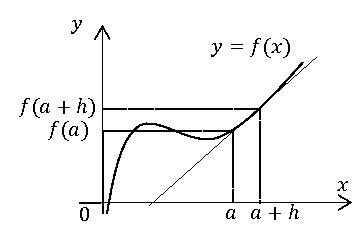
\includegraphics[bb=0 10 160 110,width=6cm]{./f_x.pdf}
  \caption{$y=f(x)$}
  \label{f_x}
 \end{minipage}
\end{figure}

$h$が十分小さい値ならば, $x=a$での接線の傾きは区間$[a, a+h]$での平均の傾きで近似できるだろう:
$$
  f'(a) = (\text{$a$における傾き})
  \approx \frac{f(a+h)-f(a)}{(a+h)-a}
  = \frac{f(a+h)-f(a)}{h}.
$$
両辺を$h$倍して移項すると
$$
f(a+h) \approx f(a) + f'(a)h.
$$
この式は$f$の点$a$における値$f(a)$と傾き$f'(a)$で$a$の付近の値を直線で近似したということを表している($h$について線形).
$a$を$x$で置き換えて
$$
f(x+h) = f(x) + f'(x)h + \epsilon
$$
と書くことにする. $\epsilon$は$h$に比べて十分小さい$h$の関数である.

さて, 二つの関数$f(x)$と$g(x)$があったとき, その積の関数$s(x)=f(x)g(x)$の微分はどうなるだろうか.
\begin{eqnarray*}
f(x+h)&=&f(x)+f'(x)h + \epsilon_1\\
g(x+h)&=&g(x)+g'(x)h + \epsilon_2
\end{eqnarray*}
を$s(x+h)$に代入して計算してみよう:
\begin{eqnarray*}
s(x+h)
 &=& f(x+h)g(x+h)
  = \left(f(x)+f'(x)h+\epsilon_1\right)\left(g(x)+g'(x)h+\epsilon_2\right)\\
 &=& f(x)g(x)+(f'(x)g(x)+f(x)g'(x))h + (h{\text より十分小さい})\\
 &=& s(x)+(f'(x)g(x)+f(x)g'(x))h + \epsilon_3
\end{eqnarray*}
となる. つまり
$$
(f(x)g(x))'=f'(x)g(x)+f(x)g'(x)
$$
が成り立つ. これが積の微分である.

もう一つ試してみよう.
今度は$y=f(x)$と$z=g(y)$という関数があったときにその合成関数$z=g(f(x))$の微分を考えてみる.
\begin{eqnarray*}
g(f(x+h))
 &=& g(f(x) + f'(x)h + \epsilon_1)
  = g(f(x)) + g'(f(x))(f'(x)h + \epsilon_1) + \epsilon_2\\
 &=& g(f(x)) + g'(f(x))f'(x)h + \epsilon_3.
\end{eqnarray*}
つまり
$$
(g(f(x)))' = g'(f(x))f'(x)
$$
が成り立つ. これは合成関数の微分である. $dy/dx=f'(x)$という微分の記号を使うと
$$
\frac{d(g(f(x)))}{dx}= \left.\frac{dg}{dy}\right|_{y=f(x)} \frac{dy}{dx}.
$$
$dy/dx$という記号があたかも約分できるように見えるのが面白い.
変数変換ではこの記法が活躍する.

\subsection{変数変換}
$$\int f(x) \,dx$$
で$x=g(y)$とすると$dx=g'(y)\,dy$より
$$\int f(g(y))\, g'(y) \,dy.$$
多変数関数の場合は$g'(y)$の部分がヤコビ行列の行列式(ヤコビアン)になる.

$x_i = g_i(y_1, \ldots, y_n) \mbox{ for $i=1, \ldots, n$}$とすると

$$\det\left(\frac{\partial (x_1, \ldots, x_n)}{\partial (y_1, \ldots, y_n)}\right) = \det\left(\diff{y_j}{x_i}\right).$$

ヤコビアンは変数変換したときのある点における微小区間の拡大率を意味する.

適当な条件の下で
\begin{eqnarray*}
& & \int \cdots \int f(x_1, \ldots, x_n)\,dx_1 \cdots \,dx_n\\
&=& \int \cdots \int f\left(g_1(y_1, \ldots, y_n), \ldots, g_n(y_1, \ldots, y_n)\right)\left|\det\left(\diff{y_j}{x_i}\right)\right|\,dy_1\cdots dy_n.
\end{eqnarray*}
\vspace{0pt}

\subsection{奇関数の積分}

全ての$x$について$f(-x)=f(x)$が成り立つとき$f$を偶関数,
$f(-x)=-f(x)$が成り立つとき$f$を奇関数という.
奇関数$f$について
$$
I:=\int_{-\infty}^\infty f(x) \,dx=0.
$$
なぜなら$I=\int_{-\infty}^0 f(x) \,dx + \int_0^\infty f(x) \,dx$と積分区間を半分にわけてみよう.
第1項で$x=-y$と変数変換すると$f(x)\,dx = -f(-y)\,dy = f(y)\,dy$となる.
積分範囲は$\infty$から$0$になり, 向きが逆転するので入れ換えると符号がひっくり返る.
よって$\text{第1項}=-\int_0^\infty f(y) \,dy$. 第2項と打ち消しあって$I=0$となるからである.
\pagebreak

$\bm{x}$が$n$次元ベクトルのときも同様に全ての$\bm{x}$について$f(-\bm{x})=-f(\bm{x})$となるとき$f$を奇関数という.
やはり
$$
I:=\int_{-\infty}^\infty \cdots \int_{-\infty}^\infty f(\bm{x}) \,dx_1 \cdots \,dx_n=0.
$$
なぜなら
$$I=\int_{-\infty}^0 \int_{-\infty}^\infty \cdots \int_{-\infty}^\infty
   +\int_0^\infty \int_{-\infty}^\infty \cdots \int_{-\infty}^\infty$$
と二つの領域に分けて$\bm{x}=-\bm{y}$と変数変換すると, $d\bm{x}=(-1)^nd\bm{y}$.
第1項の積分範囲は$(0,-\infty) \times (\infty,-\infty) \times \cdots \times (\infty,-\infty)$になり,
第2項の積分範囲に合わせると$(-1)^n$がでる.
よって$f(-\bm{y})=-f(\bm{y})$を使うと
$$I=\int_0^\infty \int_{-\infty}^\infty \cdots \int_{-\infty}^\infty f(-\bm{y})\,d\bm{y}
   +\int_0^\infty \int_{-\infty}^\infty \cdots \int_{-\infty}^\infty f(\bm{x})\,d\bm{x}=0.$$
\vspace{0pt}

\subsection{$\exp\left(-x^2\right)$の積分}

$$I:=\int_0^{\infty} \exp\left(-x^2\right) dx$$
とおくと
$$I^2=\int_0^{\infty} \int_0^{\infty} \exp\left(-(x^2 + y^2)\right) dx dy.$$
ここで$x=r\cos(\theta)$, $y=r\sin(\theta)$と置くと$x^2+y^2=r^2$.
ヤコビアンは
\begin{equation*}
\det\left(\frac{\partial (x, y)}{\partial (r, \theta)}\right) =
  \begin{vmatrix}
    \cos \theta & -r\sin \theta \\
    \sin \theta & r\cos \theta
  \end{vmatrix}
  = r(\cos^2 \theta + \sin^2 \theta) = r.
\end{equation*}

積分範囲は$x$, $y$が$(x,y)$平面の第一象限全体なので$r$は$0$から$\infty$, $\theta$は$0$から$\pi/2$を渡る.
よって
$$
  I^2
  = \int_0^{\sfrac{\pi}{2}} \int_0^\infty \exp\left(-r^2\right)r \,dr d\theta
  = \frac{\pi}{2} \left[ -\half\exp\left(-r^2\right)\right] _0^\infty
  = \frac{\pi}{4}.
$$
よって$I=\sqrt{\pi}/2$. $x^2$は偶関数なので積分範囲を$-\infty$から$\infty$にすると$2$倍になって
$$
\int_{-\infty}^\infty \exp\left(-x^2\right) \,dx = \sqrt{\pi}.
$$
本当は積分の順序を交換したりしているところを気にしないといけないが, ここでは自由に交換できるものと思っておく.

\subsection{ガウス分布の積分}

前節の積分で$a>0$をとり$x=\sqrt{a}\,y$とすると$dx=\sqrt{a}\,dy$.
$$
\int_{-\infty}^\infty \exp\left(-x^2\right) dx =\int_{-\infty}^\infty \exp\left(-ay^2\right)\sqrt{a} \,dy =\sqrt{\pi}.
$$
よって
$$
\int_{-\infty}^\infty \exp\left(-ax^2\right) dx = \sqrt{\pi/a}.
$$
ここで両辺を$a$に関して微分する.
積分の中身は$\psdif{a}\exp\left(-ax^2\right)=-x^2\exp\left(-ax^2\right)$.
気にせず積分と微分を交換することで
$$
-\int_{-\infty}^\infty x^2\exp\left(-ax^2\right) dx = -\frac{1}{2}\sqrt{\pi}a^{-3/2}.
$$
$a=1/(2\sigma^2)$と置き換えることで
\begin{equation}\label{int_exp}
\int_{-\infty}^\infty \exp\left(-\frac{1}{2\sigma^2}x^2\right) dx = \sqrt{2\pi}\sigma,
\end{equation}
\begin{equation}\label{int_xx}
\int_{-\infty}^\infty x^2\exp\left(-\frac{1}{2\sigma^2}x^2\right) dx = \sqrt{2\pi}\sigma^3.
\end{equation}
式(\ref{int_exp})は正規化項が$\sqrt{2\pi}\sigma$であることを示している.
つまりガウス分布を
$$
\fnvPair\calN(x|\mu, \sigma^2):=\frac{1}{\sqrt{2\pi}\sigma}\exp\left(-\frac{1}{2\sigma^2}(x-\mu)^2\right)
$$
とすると
$$
\int_{-\infty}^\infty \fnvPair\calN(x|\mu, \sigma^2) dx=1.
$$
平均は
$$
x \,\fnvPair\calN(x|\mu, \sigma^2)
= (x-\mu) \,\fnvPair\calN(x|\mu, \sigma^2)
  + \mu \,\fnvPair\calN(x|\mu, \sigma^2)
$$
とわけると, 第1項は$(x-\mu)$に関して奇関数なので積分すると消えて
$$
\EE[x]:=\int_{-\infty}^\infty x \,\fnvPair\calN(x|\mu, \sigma^2) dx=\mu.
$$
分散は
$$
\var[x]:=\EE[(x-\mu)^2]=\int_{-\infty}^\infty (x-\mu)^2 \,\fnvPair\calN(x|\mu, \sigma^2) dx.
$$
$y=x-\mu$と変数変換すると式(\ref{int_xx})の左辺を正規化項$\sqrt{2\pi}\sigma$で割ったものとなり,
$$
\EE[(x-\mu)^2]=\sigma^2.
$$
%\vspace{0pt}

\section{線形代数の復習}
\subsection{行列の積}
以下, 特に断らない限り行列の数値は複素数とする.

$A$を$m$行$n$列の行列とする. 横に$n$個, 縦に$m$個数字が並んでいる. $A$の$i$行$j$列の値が$a_{ij}$であるとき, $A=(a_{ij})$と書く. $m=n$のとき$n$次正方行列という. 並んでいる数字が実数値のみからなる行列を実行列という.

$A$を$l$行$m$列の行列, $B$を$m$行$n$列の行列とするとき, 積$AB$を$(AB)_{ij} := \sum_{k=1}^n a_{ik} b_{kj}$で定義する. $AB$は$l$行$n$列の行列になる.

\begin{enumerate}
\item $A$, $B$が正方行列だったとしても$AB=BA$とは限らない.
\item $A$, $B$, $C$がその順序で掛け算できるとき$(AB)C=A(BC)$が成り立つ.\\
なぜなら
$\left((AB)C\right)_{ij}=\sum_k (AB)_{ik} c_{kj} = \sum_k \left(\sum_l a_{il}b_{lk}\right) c_{kj} = \sum_{k,l} a_{il}b_{lk}c_{kj}$.\\
$A(BC)_{ij}=\sum_l a_{il} (BC)_{lj} = \sum_l a_{il} \left(\sum_k b_{lk}c_{kj}\right) = \sum_{k,l} a_{il}b_{lk}c_{kj}$だから.
\end{enumerate}
\vspace{0pt}

\subsection{トレース}

$A$が$n$次正方行列のとき$\tr(A) := \sum_{i=1}^n a_{ii}$と$A$のトレースと呼ぶ.
$$
\tr(A+B)=\tr(A) + \tr(B).
$$
$$
\tr(AB)=\tr(BA).
$$
なぜなら$\tr(AB)=\sum_i (AB)_{ii}=\sum_i \left(\sum_j a_{ij}b_{ji}\right)=\sum_j \left(\sum_i b_{ji}a_{ij}\right)=\sum_j (BA)_{jj}=\tr(BA).$
3個の行列の積については
$
\tr(ABC)=\sum_i (ABC)_{ii} = \sum_i \left(\sum_{j,k} a_{ij} b_{jk} c_{ki}\right) = \sum_{i,j,k} a_{ij} b_{jk} c_{ki}
$
より
$$
\tr(ABC)=\tr(BCA)=\tr(CAB).
$$
$\displaystyle A = \matt{a}{b}{c}{d}$のときは$\tr(A)=a+d$.
\vspace{\baselineskip}

\subsection{行列式}
$$A = \matt{a}{b}{c}{d}$$
のとき, $\det(A):=ad-bc$を$A$の行列式という. $|A|$とも書く.
$|A|$は絶対値の記号ではないので$0$以上とは限らないことに注意する.
一般には次のように定義する:

$S_n$を$1,\ldots,n$の順序を並び替える操作全体の集合とする. たとえば$S_2$は何も動かさない操作と$1$を$2$に, $2$を$1$に並び替える操作の二つの操作からなる. $n$個の要素を並び替える組み合わせは$n \times (n-1) \times \cdots \times 1 = n!$通りある.

$D:=\prod_{i<j}(x_i - x_j)$とし, $S_n \ni \sigma$に対して$\sigma D := \prod_{i<j}\left(x_{\sigma(i)} - x_{\sigma(j)}\right)$とすると,$D$と$\sigma D$は符号しか変わらない. $\sigma D = \sgn(\sigma) D$で$\sgn(\sigma) \in \{1,-1\}$を定義する.

$\{\sigma(1), \ldots, \sigma(n)\}$を2個ずつ順序を入れ換えて$\{1, \ldots, n\}$に並び替えられたとき, 偶数回でできたら$\sgn(\sigma)=1$, 奇数回でできたら$\sgn(\sigma)=-1$である.
これを使って行列式を定義する.

$A$を$n$次正方行列($n$行$n$列)とするとき,
$$\det(A):=\sum_{\sigma \in S_n} \sgn(\sigma)\, a_{1 \sigma(1)} \cdots a_{n \sigma(n)}.$$

$A$が2次正方行列のときを見直してみる. $S_2$は$2$個の要素しかもたなかった. 一つは何も動かさない操作でそれに対して$\sgn$は1.
もう一つは$1$と$2$を入れ換える操作で$\sgn$は$-1$となる. よって
$$
\det(A)=|A|= a_{1 1} a_{2 2} - a_{1 2} a_{2 1}.
$$
ここで二つの$n$次正方行列$A$, $B$に対して$|AB|=|A||B|$が成り立つ. 2次のときのみ確認しておこう.
$$
  A = \matt{a}{b}{c}{d}
  ,\hseq
  B = \matt{x}{y}{z}{w}
$$
とするとき,
\begin{eqnarray*}
|AB|
 &=& \matt{ax+bz}{ay+bw}{cx+dz}{cy+dw}
  = (ax+bz)(cy+dw)-(ay+bw)(cx+dz) \\
 &=& (ad-bc)(xw-yz)
  = \dett{a}{b}{c}{d} \dett{x}{y}{z}{w}
  = |A||B|.
\end{eqnarray*}
一般のときの証明は省略する.

\subsection{行列の種類}

$A$を$m$行$n$列の行列とする. $A$に対して$\trans{A} := (a_{ji})$を$A$の転置行列という.
これは$n$行$m$列の行列である.
$\det(\trans{A})=\det(A)$, $\trans{(AB)}=\trans{B}\trans{A}$である.

$x$, $y \in \RR$として$z:=x+y\sqrt{-1} \in \CC$に対し$\overline{z}:=x-y\sqrt{-1}$を$z$の複素共役という.
$a_{ij}\in \CC$のとき, $\overline{A}:=(\overline{a_{ij}})$を$A$の複素共役行列,
$A^*:=\overline{\trans{A}}$を随伴行列という.
$\det(\overline{A})=\overline{\det(A)}$, $\det(A^*)=\overline{\det(A)}$, $(AB)^*=B^* A^*$である.

$A$が$n$次正方行列のとき, $a_{ii}$を対角成分という.
対角成分以外の項が$0$である行列を対角行列といい $\diag(a_1, \ldots, a_n)$と書く.
また,
$$
\delta_{ij}:=
\begin{cases}
1 & (i = j), \\
0 & (i \neq j)
\end{cases}
$$
をクロネッカーの$\delta$といい,
$I_n:=(\delta_{ij})$を$n$次単位行列という. $I$と略すこともあるし$E$と書くこともある.
このとき$AI_n=I_nA=A$である.

$A$が$n$次正方行列で, $\det(A)\neq0$のとき$A$を正則といい, $AB=BA=I$となる行列$B$が存在する.
$B$を逆行列といい, $A^{-1}$と書く.

\begin{enumerate}
\item 逆行列は存在すればただ一つである. なぜなら$B$, $B'$を逆行列とすると$B=BI=B(AB')=(BA)B'=IB'=B'$.
\item 有限次元では$AB=I$ならば$BA=I$である(証明は略).つまり$AB=I$だが$BA\neq I$なものは存在しない(無限次元ではそのような行列を構成できる).
\end{enumerate}

$n$次正方行列$A$について

\begin{enumerate}
\item $\det(A) \neq 0$なもの全体を$GL_n(\CC)$と書く. 実正則行列全体は$GL_n(\RR)$と書く.
\item $\det(A)=1$なもの全体を$SL_n(\CC)$と書く. 実行列のときは$SL_n(\RR)$.
\item $AA^*=I$となるときユニタリー行列といい, その全体を$U(n)$と書く. このとき$|AA^*|=|\det(A)|^2=1$.
ここで$|\det(A)|$は$\det(A)$の(複素数としての)絶対値である.
ユニタリー行列であって, 更に$\det(A)=1$なもの全体を$SU(n)$と書く.
\item 実行列$A$が$A\trans{A}=I$となるとき, 直交行列といい, その全体を$O(n)$と書く. このとき$|\det(A)|^2=1$.
$\det(A) \in \RR$なので$\det(A)=\pm 1$.
$\det(A)=1$なもの全体を$SO(n)$と書く.
\item $A=\trans{A}$となるとき対称行列という.
\end{enumerate}
\vspace{0pt}

\subsection{ブロック行列の逆行列}

$A$, $D$を正方行列として($B$, $C$は正方行列とは限らない)
$$
X:=\matt{A}{B}{C}{D}
$$
の逆行列を求めてみよう.
逆行列を
$$
X^{-1}=\matt{M}{N}{L}{P}
$$
とおくと
$$
\matt{A}{B}{C}{D} \matt{M}{N}{L}{P}=\matt{AM+BL}{AN+BP}{CM+DL}{CN+DP}=\matt{I}{0}{0}{I}.
$$
2-1ブロックに左から$D^{-1}$を掛けて$L=-D^{-1}CM$.
これを1-1ブロックに代入して
$$
AM+BL=AM-BD^{-1}CM=(A-BD^{-1}C)M=I.
$$
よって$M=(A-BD^{-1}C)^{-1}$.
今度は
$$\matt{M}{N}{L}{P} \matt{A}{B}{C}{D}=\matt{MA+NC}{MB+ND}{LA+PC}{LB+PD}=\matt{I}{0}{0}{I}$$
の1-2ブロックに右から$D^{-1}$を掛けて$N=-MBD^{-1}$.

2-2ブロックに右から$D^{-1}$を掛けて$P=D^{-1}-LBD^{-1}=D^{-1}+D^{-1}CMBD^{-1}$.

よって$M=(A-BD^{-1}C)^{-1}$として
$$\matt{M}{N}{L}{P}=\matt{M}{-MBD^{-1}}{-D^{-1}CM}{D^{-1}+D^{-1}CMBD^{-1}}.$$
これが$X$の逆行列となることは容易に確認できる.

(以下余談)
$R=MB$, $S=D^{-1}C$とおくと
$$X=\matt{M^{-1}}{0}{0}{D} \matt{I+MBD^{-1}C}{MB}{D^{-1}C}{I}=\matt{M^{-1}}{0}{0}{D}\matt{I+RS}{R}{S}{I}$$
と変形できることはすぐ分かる.
$$
\matt{M^{-1}}{0}{0}{D}^{-1}=\matt{M}{0}{0}{D^{-1}}
,\hseq
\matt{I+RS}{R}{S}{I}^{-1}=\matt{I}{-R}{-S}{I+SR}
$$
なので$X^{-1}$もすぐ求められる. 更にこの行列の行列式は$1$なので
$$
|X|=\dett{M^{-1}}{0}{0}{D} = |M|^{-1}|D|=|A-BD^{-1}C||D|.
$$
\vspace{0pt}

\subsection{三角化}

$n$次正方行列$A$に対して$a_{ij} = 0\ (i>j)$のとき(上半)三角行列という.
$$A=\lmatt{a_{11}}{*}{0}{a_{nn}}.$$
ここの$*$は任意の値が入っていることを示す.

このとき$\det(A)=\prod_i a_{ii}$である. なぜなら行列式の定義で1行ごとに異なる列のものをとっていったものの積を考えるわけだが,
最初に$a_{11}$以外の$a_{1j} (j>1)$を選択すると, 残り$n-1$個をとる中で$0$でないものは$n-2$個しかない. したがって必ず$0$になる.
以下同様にして対角成分を拾ったものしか残らないからである.

さて次の定理を証明無しで認める:
\begin{thm}\label{trigonal}
任意のn次正方行列Aに対して, あるユニタリー行列$P$があって$P^{-1}AP$を三角化できる.
\end{thm}
(注意)一般の行列が常に対角化できるとは限らないが三角化は常にできる.

\subsection{対称行列}

\begin{thm}
$n$次実対称行列$A$に対して, ある行列$P$が存在して$P^{-1}AP$を実対角化できる.
\end{thm}

定理\ref{trigonal}を用いてこの定理を証明しよう.

$A$に対してあるユニタリー行列$P$があって$P^{-1}AP$を三角化できる:
$$P^{-1}AP=
\begin{pmatrix}
  \lambda_1 & \ldots & * \\
  \vdots & \ddots & \vdots \\
  0 & \ldots & \lambda_n
\end{pmatrix}.
$$
この両辺の随伴をとる. $P$はユニタリー行列なので$PP^*=I$. つまり$P^{-1} = P^*$.
さらに$A$は実対称行列なので$A^*=A$に注意すると
$$P^*A^*(P^{-1})^*=P^{-1}AP=
\begin{pmatrix}
  \overline{\lambda_1} & \ldots & 0 \\
  \vdots & \ddots & \vdots \\
  * & \ldots & \overline{\lambda_n}
\end{pmatrix}.
$$
この二つの式が同一なので$\overline{\lambda_i}=\lambda_i$かつ$*$の部分が$0$.
これは$\lambda_i \in \RR$で, $P^{-1}AP$はもともと対角行列であったことを意味する.

実は$P$が実行列であるようにもできる. そのとき$P$は直交行列となり$\det(P)=\pm 1$.

もし$\det(P)=-1$だったとすると, $I'$を単位行列の$1$行目と$2$行目を入れ換えたものとして$P'=PI'$とおいて
$$P'^{-1}AP'=I'(P^{-1}AP)I'=I'\diag(\lambda_1, \ldots, \lambda_n)I'
=\diag(\lambda_2, \lambda_1, \lambda_3, \dots, \lambda_n).$$
これはもとの対角成分の1番目と2番目を入れ換えたものである.
$\det(I')=-1$, $\det(P')=\det(P)\det(I')=1$なのでもともと$\det(P)=1$だったとしてもよい.
従ってより強く次の定理が成り立つ.
\begin{thm}\label{sym}
$n$次実対称行列$A$に対して, ある$P \in SO(n)$が存在して$P^{-1}AP$を実対角化できる.
\end{thm}
なお, PRMLでは直交行列の行列式が$1$であることを暗に仮定しているときがあるが不正確(cf. (C.37)付近).
たとえばPRML 式(2.54)で$\det(J)^2=1$から$\det(J)=1$を出しているが, $\det(J)=-1$の可能性もある.
予め$U$を$SO(n)$の元としてとっておけば
$$
\det(J)=\det(U)=1
$$
\pagebreak
ですむ.
ただし多重積分を考えるときはヤコビアンの絶対値のみが関係するのでここでは$|\det(J)|=1$が言えれば十分である.

\subsection{2次形式}

$A$を一般に$n$次正方行列とし, $\bm{x}$を$n$次元縦ベクトルとする.
\begin{equation}\label{square_form}
\quadf{A}{x} = \sum_i x_i \left(A \bm{x}\right)_i = \sum_i x_i \left(\sum_j a_{ij} x_j\right) = \sum_{i,j} a_{ij} x_i x_j
\end{equation}
を$x$の2次形式という.

$A$が与えられたときに$S=(A+\trans{A})/2$, $T=(A-\trans{A})/2$とすると,
$A=S+T$, $\trans{S}=S$, $\trans{T}=-T$となる.
$\trans{T}=-T$ということは$t_{ij}=-t_{ji}$なので(標数$2$ではないから)$t_{ii}=0$.
式(\ref{square_form})の和を$i=j$と$i\neq j$の二つに分けて$A=T$として適用すると
$$\quadf{T}{x} = \sum_i t_{ii} x_i x_j + \sum_{i<j} (t_{ij} + t_{ji}) x_i x_y.$$

第1項は$t_{ii}=0$より$0$. 第2項も$t_{ij}=-t_{ji}$より$0$.
つまり$\trans{T}=-T$のとき2次形式の値は$0$となる.
よって$\quadf{A}{x} = \quadf{S}{x} + \quadf{T}{x} = \quadf{S}{x}$.
つまり2次形式を考えるときは一般性を失うことなく$A$を対称行列としてよい.

2変数のときを見てみる. 行列の計算は分かりにくければとりあえず2次で書いてみること.
$$
\trans{\vvec{x}{y}}\matt{a}{b}{b}{c}\vvec{x}{y}
=\hvec{x}{y}\vvec{ax+by}{bx+cy}=ax^2+2bxy+cy^2.
$$
ブロック行列なら$A$, $C$を対称行列として
$$
\trans{\vvec{\bm{x}}{\bm{y}}}\matt{A}{B}{{\trans{B}}}{C}\vvec{\bm{x}}{\bm{y}}
 =\hvec{\trans{\bm{x}}}{\trans{\bm{y}}}\vvec{A\bm{x}+B\bm{y}}{\trans{B}\bm{x}+C\bm{y}}
 =\quadf{A}{x}+2\trans{\bm{x}}B\bm{y}+\quadf{C}{y}.
$$
ここで$\trans{\bm{x}}B\bm{y}$はスカラー値なので転置しても変わらない,
つまり
$$
\trans{\bm{x}}B\bm{y}
=\trans{(\trans{\bm{x}}B\bm{y})}
=\trans{\bm{y}}\trans{B}\trans{(\trans{\bm{x}})}
=\trans{\bm{y}}\trans{B}\bm{x}
$$
を用いた.
対称行列は$SO(n)$の元$P$を用いて対角化できた($P\trans{P}=I$).
$\bm{y}=P^{-1}\bm{x}$とおくと
$$
\quadf{A}{x}
=\trans{\bm{y}}\trans{P}AP\bm{y}
=\quadf{\diag(\lambda_1,\ldots,\lambda_n)}{y}=\sum_{i=1}^n \lambda_i y_i^2.
$$
つまり2次形式は対角化すれば単なる成分ごとの直和になる.

\section{多変量ガウス分布}

$A$を$n$次実対称行列, $\bm{x}$を$n$次元縦ベクトルとする.
まず
$$
f(\bm{x}):=\exp\left(-\half\quadf{A^{-1}}{x}\right)
$$
を考える.
これは$\bm{x}$について偶関数である.
$A$を直交行列$P$で対角化する.
$P^{-1}AP=\diag(\lambda_1, \ldots, \lambda_n)$より, $P^{-1}A^{-1}P=\diag(\lambda_1^{-1}, \ldots, \lambda_n^{-1}).$
$\bm{y}=P^{-1}\bm{x}$と置いて前節の変形を行うと
$$f(\bm{x})
=\exp\left(-\half\sum_{i=1}^n \frac{y_i^2}{\lambda_i}\right)
=\prod_{i=1}^n\exp\left(-\frac{y_i^2}{2\lambda_i}\right).$$
ここで区間$(-\infty,\infty)$の積分を考えるが, そうすると積分値が発散しないためには
全ての$\lambda_i>0$である必要がある. 以下この条件を仮定する.
このとき$|A|=\prod_i \lambda_i>0$.

積分値は式(\ref{int_exp})より
$$
\int f(\bm{x})\,d\bm{x}
=\int f(P\bm{y})
 \underbrace{\left|\det\frac{\partial \bm{x}}{\partial \bm{y}}\right|}
 _{= \mathopen|\det P\mathclose| = 1}
 d\bm{y}
=\prod_{i=1}^n \sqrt{2\pi\lambda_i} = (2\pi)^{\sfrac{n}{2}} \sqrt{|A|}.
$$
よって
$$
\fnvPair\calN(\bm{x}|\bm{\mu}, A)
  :=\frac{f(\bm{x}-\bm{\mu})}{(2\pi)^{\sfrac{n}{2}} \sqrt{|A|}}
  =\frac1{(2\pi)^{\sfrac{n}{2}}} \frac{1}{\sqrt{|A|}}\exp\left(-\half\trans{(\bm{x-\mu})}A^{-1}(\bm{x-\mu})\right)
$$
とすると正規化されている.
これが多変量版のガウス分布である.

平均値$\EE[\bm{x}]$を求めよう:
$$
\bm{x}f(\bm{x}-\bm{\mu})
 =(\bm{x}-\bm{\mu})f(\bm{x}-\bm{\mu}) + \bm{\mu}f(\bm{x}-\bm{\mu})
$$
とすると第1項は$(\bm{x}-\bm{\mu})$に関して奇関数なので積分すると消える.
第2項は$\bm{\mu}$が定数で外に出るので
$$
\EE[\bm{x}]
= \int \bm{x}\, \fnvPair\calN(\bm{x}|\bm{\mu}, A) d\bm{x}
= \bm{\mu}.
$$

次に分散$\var[\bm{x}]=\EE[(\bm{x}-\bm{\mu})\trans{(\bm{x}-\bm{\mu})}]$を求めよう:
$\bm{y}$を$P\bm{y} = \bm{x}-\bm{\mu}$となるようにおくと
$$
(\bm{x}-\bm{\mu})\trans{(\bm{x}-\bm{\mu})}=P\bm{y}\trans{\bm{y}}\trans{P}.
$$
$P=(\bm{p_1}, \ldots, \bm{p_n})$とすると
$(P\bm{y})_i = \sum_{j=1}^n p_{ij} y_j$だから
$$P\bm{y} = \sum_{j=1}^n y_j \bm{p_j}.$$
よって
$$
P\bm{y}\trans{\bm{y}}\trans{P} \times f(\bm{x}-\bm{\mu})
=
\sum_{i,j}
  \bm{p_i}\trans{\bm{p_j}} y_i y_j
  \prod_{k=1}^n \exp\left(-\frac{y_k^2}{2\lambda_k}\right).
$$
積分すると$i\neq j$のところでは
$y_i \exp\left(-\sfrac{y_i^2}{(2\lambda_i)}\right)$が奇関数になるので$0$.
$i=j$のところでは,
$k=i$のときに$y_i^2 \exp\left(-\sfrac{y_i^2}{(2\lambda_i)}\right)$から
$\lambda_i\sqrt{2\pi\lambda_i}$がでて,
それ以外の$k\neq i$のときに$\sqrt{2\pi\lambda_k}$がでる.
つまり全体で$\lambda_i \prod_{k=1}^n(\sqrt{2\pi\lambda_k})=\lambda_i \times \text{正規化項}$.
よって
\begin{eqnarray*}
&&
\var[\bm{x}] =
\EE[P\bm{y}\trans{\bm{y}}\trans{P}]
 = \int P\bm{y}\trans{\bm{y}}\trans{P}
   \fnvPair\calN(\bm{x}|\bm{\mu}, A) d\bm{x}
 = \sum_i \bm{p_i}\trans{\bm{p_i}} \lambda_i
\\
&& \hseq
 = (\bm{p_1}, \ldots, \bm{p_n}) \diag(\lambda_1, \ldots, \lambda_n)
\begin{pmatrix}
\trans{\bm{p_1}} \\
\vdots \\
\trans{\bm{p_n}}
\end{pmatrix}
= P \diag(\lambda_1, \ldots, \lambda_n) \trans{P}
= A.
\end{eqnarray*}
\vspace{0pt}

\section{行列の微分}
ここではガウス分布の最尤推定で使ういくつかの公式を列挙する.
PRMLの付録Cではたとえば(C.22)を(C.33)や(C.47)を使って示せとあるが,
それだと対称行列や対角化ができる行列に対してしか示せていない中途半端なものである.
これらはもっと一般的な行列で成り立つ.

$A$を$n$次正方行列とする.

\subsection{2次形式の別の表現}
$\bm{x}$を$n$次縦ベクトルとするとき,
\begin{equation}\label{quad}
\quadf{A}{x}=\sum_{i,j} a_{ij} x_i x_j=\sum_i \left(\sum_j a_{ij} (\bm{x}\trans{\bm{x}})_{ji}\right)=\sum_i (A \bm{x}\trans{\bm{x}})_{ii}=\tr(A \bm{x}\trans{\bm{x}}).
\end{equation}
この式は$A$が対称行列でなくても成り立つことに注意する.

\subsection{内積の微分}
$\bm{x}$, $\bm{y}$を縦ベクトルとして
$$
\dif{\bm{x}} \left(\trans{\bm{x}}\bm{y}\right) = \bm{y},\hseq
\dif{\bm{y}} \left(\trans{\bm{x}}\bm{y}\right) = \bm{x}.
$$
\pagebreak
ここで$\sdif{\bm{x}}$は$\sdif{x_i}$を縦に並べた縦ベクトルとする.
$\sdif{\bm{x}}$を$\nabla$と書くこともあるがPRMLでは場所によって
縦ベクトル(2.228)だったり, 横ベクトル(3.13)だったりする.
常に縦ベクトルとしたほうが混乱は少ない.

証明は$\trans{\bm{x}}\bm{y}=\sum_j x_j y_j$なので
\begin{eqnarray*}&&
\dif{x_i}\left(\trans{\bm{x}}\bm{y}\right)=\sum_j \delta_{ij} y_j=y_j,\hseq
\dif{y_i}\left(\trans{\bm{x}}\bm{y}\right)=\sum_j x_j \delta_{ij}=x_j.
\end{eqnarray*}
\vspace{0pt}

\subsection{2次形式の微分}
\begin{equation}\label{diff_quad}
\dif{\bm{x}}\left(\quadf{A}{x}\right)=(A+\trans{A})\bm{x}.
\end{equation}
証明は
\begin{eqnarray*}
\dif{x_i}\left(\quadf{A}{x}\right)
&=& \sum_{s,t} a_{st} \dif{x_i}(x_s x_t)= \sum_{s,t} a_{st} (\delta_{is} x_t + x_s \delta_{it})\\
&=& \left(\sum_t a_{it} x_t\right) + \left(\sum_s a_{si} x_s\right)
= (A\bm{x})_i + (\trans{A}\bm{x})_i = \left((A + \trans{A})\,\bm{x}\right)_i.
\end{eqnarray*}
特に$A$が対称行列のときは
$$\dif{\bm{x}}\left(\quadf{A}{x}\right)=2A\bm{x}.$$
\vspace{0pt}

\subsection{逆行列の微分}
$AA^{-1}=I$の両辺を$x$で微分すると
$$\left(\dif{x} A\right)A^{-1}+A \dif{x}\left(A^{-1}\right)=0.$$
左から$A^{-1}$をかけることによって
\begin{equation}\label{diff_inv}
\dif{x}\left(A^{-1}\right)=-A^{-1}\left(\dif{x} A\right)A^{-1}.
\end{equation}
\vspace{0pt}

\subsection{行列式の対数の微分の公式(1)}
$|A|>0$となる行列に対して
$$
\dif{x}\log |A| = \tr\left(A^{-1} \dif{x} A\right).
$$
(証明)$A$を$P$で三角化する.
$$
A=P^{-1}\lmatt{\lambda_1}{*}{0}{\lambda_n}P.
$$
ここで計算を見やすくするために
$$\lmatt{\lambda_1}{*}{0}{\lambda_n}=\tri(\lambda_i)$$
と略記する.
すると上の式は
$$A=P^{-1}\tri(\lambda_i)P$$
と表記できる.
逆行列は
$$A^{-1}=P^{-1}\tri(\lambda_i)^{-1}P$$
となる.
さて$|A|=\prod \lambda_i$なので証明すべき式の左辺は
$$
\dif{x}\left(\sum \log (\lambda_i)\right) = \sum \frac{\lambda_i'}{\lambda_i}.
$$
ここで$\diff{x}{\lambda_i}=\lambda_i'$と略記した.
証明すべき右辺を考えよう.
\pagebreak
$$
\diff{x}{A}
 =A'
 =\left(P^{-1}\tri(\lambda_i)P\right)'
 =(P^{-1})'\tri(\lambda_i)P + P^{-1}\tri(\lambda_i')P + P^{-1}\tri(\lambda_i)P'.
$$
第1項に式(\ref{diff_inv})を使うと
$$
(P^{-1})'\tri(\lambda_i)P=-P^{-1}P'P^{-1}\tri(\lambda_i)P
$$
更に$\tr(A+B)=\tr(A)+\tr(B)$を使うと
\begin{eqnarray*}
\tr\left(A^{-1}A'\right)
 &=& -\tr\left(\left(P^{-1}\tri(\lambda_i)^{-1}P\right)P^{-1}P'P^{-1}\tri(\lambda_i)P\right)\\
 & & +\tr\left((P^{-1}\tri(\lambda_i)^{-1}P)P^{-1}\tri(\lambda_i')P\right)\\
 & & +\tr\left((P^{-1}\tri(\lambda_i)^{-1}P)P^{-1}\tri(\lambda_i)P'\right)\\
 &=& -\tr\left(P^{-1}\tri(\lambda_i)^{-1}P'P^{-1}\tri(\lambda_i)P\right)\\
 & & +\tr\left(P^{-1}\tri(\lambda_i)^{-1}\tri(\lambda_i')P\right)\\
 & & +\tr(P^{-1}P').
\end{eqnarray*}
次に$\tr(AB)=\tr(BA)$を使ってトレースの中の積の順序を入れ換えて,
行列と逆行列の積を消していくと
\begin{eqnarray*}
\tr(A^{-1}A')
 &=& -\tr\left(P'P^{-1}\tri(\lambda_i)PP^{-1}\tri(\lambda_i^{-1})\right)
     +\tr\left(\tri(\lambda_i)^{-1}\tri(\lambda_i')PP^{-1}\right)\\
 & & +\tr(P^{-1}P')\\
 &=&-\tr(P'P^{-1})+\tr(\tri(\lambda_i)^{-1}\tri(\lambda_i'))+\tr(P^{-1}P')\\
 &=&\tr\left(\tri(\lambda_i)^{-1}\tri(\lambda_i')\right).
\end{eqnarray*}
三角行列の逆行列はやはり三角行列であり,
$*$の部分はもとの行列の部分とは異なる何かわからない値になる.
しかし対角成分はもとの対角成分の逆数が並ぶ.
つまり
$$
\tri(\lambda_i)^{-1}=\tri(\lambda_i^{-1}).
$$
よって
$$
\tr(A^{-1}A')
 =\tr\left(\tri(\lambda_i^{-1}\lambda_i')\right)=\sum \frac{\lambda_i'}{\lambda_i}.
$$
これで左辺$=$右辺が示された.

\subsection{行列式の対数の微分の公式(2)}
$|A|>0$となる行列に対して
\begin{equation}\label{diff_log_mat}
\dif{A}\log |A| = \trans{{(A^{-1})}}.
\end{equation}
ここで行列$A$で微分するというのは各要素$a_{ij}$で微分したものを,
行列に並べたものを意味する.
今示した対数の微分の公式(1)より
$$\dif{a_{ij}}\log|A|=\tr\left(A^{-1}\dif{a_{ij}}A\right).$$
$\partial A / \partial a_{ij}$は$ij$成分のみが$1$でそれ以外は$0$の行列になる.
その行列を$I_{ij}$と書くと,
\begin{eqnarray*}
\tr(A^{-1}I_{ij})
 &=&\sum_s \left(A^{-1}I_{ij}\right)_{ss}
 = \sum_s \left(\sum_t (A^{-1})_{st} (I_{ij})_{ts}\right)
 = \sum_s \left(\sum_t (A^{-1})_{st} \delta_{it} \delta_{js}\right)\\
 &=& (A^{-1})_{ji}.
\end{eqnarray*}
つまり$\log|A|$を$a_{ij}$成分で微分すると
$A^{-1}$の$ji$成分になることが分かったので証明完了.

実はこの式は三角化を使わなくても行列式の定義から直接示すことができる.
2次正方行列で示してみよう.
$A=\matt{a}{b}{c}{d}$とすると$|A|=ad-bc$.
よって左辺は$\log|A|$を$a$, $b$, $c$, $d$でそれぞれ微分して
$$
\text{左辺}=\frac{1}{|A|}\matt{d}{-c}{-b}{a}=\text{右辺}.
$$
一般のときは$|A|=\sum_{\sigma \in S_n} \sgn(\sigma)\, a_{1 \sigma(1)} \cdots a_{n \sigma(n)}$なので
$$
|A|(\text{左辺})_{ij}=\sum_{\sigma \in S_n} \sgn(\sigma) \dif{a_{ij}}\left(a_{1 \sigma(1)} \cdots a_{n \sigma(n)}\right).
$$
$a_{ij}$による微分を考えると, 掛け算の中に$a_{ij}$があれば(微分が$1$なので)それを取り除き,
なければ$0$になってしまう.
$a_{ij}$が現れるのは$j=\sigma(i)$を固定する$\sigma$についてのみである.
つまり行列$A$から$i$行$j$列を取り除いたものになる.

実はこの式は$A$の余因子行列$\tilde{A}$の余因子$\tilde{A}_{ji}$と呼ばれるもので,
$$A\tilde{A}=|A|\,I$$
となることが示される(というか順序が逆で, 普通は逆行列をこれで構成する).
つまり$\text{左辺}=\trans{{(A^{-1})}}$.

\section{ガウス分布の最尤推定}
多変量ガウス分布から, $N$個の観測値$\bm{X}=\{\bm{x_i}\}$が独立に得られたときに,
対数尤度関数
$$\log \fnvPair p(\bm{X}|\bm{\mu}, A)
:=-\frac{Nn}{2}\log(2\pi)-\frac{N}{2}\log|A|-\half\sum_{i=1}^N \trans{(\bm{x_i-\mu})}A^{-1}(\bm{x_i-\mu})$$
を最大化する$A$を求めよう. PRML(演習2.34)では「対称性を仮定せずに解いた結果が対称であった」という方針で解けと記されている.
しかし, その導出過程で対称性を利用しているのはおかしい.
ここでは$A$の対称性を仮定せずに話を進める.

その前にまず$A$を固定したときの$\bm{\mu}$に関する最尤推定の解を求めておこう.
式(\ref{diff_quad})より
\begin{eqnarray*}
\dif{\bm{\mu}} \log \fnvPair p(\bm{X}|\bm{\mu}, A)
&=&\half\sum_{i=1}^N\left(A^{-1}+\trans{(A^{-1})}\right)(\bm{x_i-\mu})\\
&=&\half\left(A^{-1}+\trans{(A^{-1})}\right)\left(\left(\sum_{i=1}^N \bm{x_i}\right) - N\bm{\mu}\right).
\end{eqnarray*}
これが$\bm{0}$なので
$$
\bm{\mu}_{\text{ML}}:=\frac{1}{N}\sum_i \bm{x_i}.
$$
さて, 本題に戻る. 再び$A$が対称行列でないという仮定に注意して式を変形する.
$\bm{y_i}=\bm{x_i}-\bm{\mu}$とおき
$$
F(A):=-N\log|A|-\sum_i \quadf{A^{-1}}{y_i}
=-N\log|A|-\tr\left(A^{-1}\sum_i \bm{y_i}\trans{\bm{y_i}}\right)
$$
とおく.
第2項の式変形には式(\ref{quad})を用いた.
$B=\sum_i \bm{y_i}\trans{\bm{y_i}}$と置いて$A$で微分しよう.
第1項は式(\ref{diff_log_mat})を使って$-N\trans{{(A^{-1})}}$.
第2項を求めるには式(\ref{diff_inv})を使って
\begin{eqnarray*}
\dif{a_{ij}}\tr\left(A^{-1}B\right)
 &=& \tr\left(\left(\dif{a_{ij}}A^{-1}\right)B\right)
 = -\tr\left(A^{-1}\left(\dif{a_{ij}}A\right)A^{-1}B\right)\\
&=&-\tr\left(\left(\dif{a_{ij}}A\right)A^{-1}BA^{-1}\right).
\end{eqnarray*}
最後の式変形では$\tr(XY)=\tr(YX)$を使った. $C=A^{-1}BA^{-1}$とおく.
\begin{eqnarray*}
\tr\left(\left(\dif{a_{ij}}A\right)C\right)
 &=& \sum_s \left(\left(\dif{a_{ij}}A\right)C\right)_{ss}
  = \sum_s \left(\sum_t \left(\dif{a_{ij}}A\right)_{st} c_{ts}\right)\\
 &=& \sum_{s,t} \delta_{is} \delta_{jt} c_{ts}=c_{ji}.
\end{eqnarray*}
つまり
\begin{eqnarray}\label{diff_tr_invA_B}
\dif{A}\tr(A^{-1}B)=-\trans{C}=-\trans{(A^{-1}BA^{-1})}.
\end{eqnarray}
よって
$$\dif{A}F(A)=-N\trans{{(A^{-1})}}+\trans{(A^{-1}BA^{-1})}.$$
これが$0$になるような$A$が$F(A)$の最大値を与える.
転置をとって
$$
-NA^{-1}+A^{-1}BA^{-1}=0.
$$
$$
A
 =\frac{1}{N}B
 =\frac{1}{N}\sum_i \bm{y_i}\trans{\bm{y_i}}
 =\frac{1}{N}\sum_i (\bm{x_i}-\bm{\mu})\trans{(\bm{x_i}-\bm{\mu})}.
$$
この$A$は明らかに対称行列である.
つまり$A$に関する対称性を仮定せずに最尤解を求めると$A$が対称行列となることが分かった.
また, $\bm{\mu}$について特に条件も無いので,
先に$\bm{\mu}$に関して最尤推定による解$\bm{\mu}_{\text{ML}}$を代入すれば,
この$\bm{\mu}$と$A$の組が$\fnvPair p(\bm x|\bm\mu, A)$を最大化することが分かる.
